3. $\cfrac{x(x^2+2)(2-x)(x^3-64)}{(x^2-16)(x+2)^2}\leqslant 0 \Leftrightarrow \cfrac{x(2-x)(x-4)(x^2+4x+16)}{(x-4)(x+4)(x+2)^2}\leqslant 0.$ Применив метод интервалов, найдём ответ: $x\in(-4;-2)\cup(-2;0]\cup[2;4)\cup(4;+\infty).$
\begin{figure}[ht!]
\center{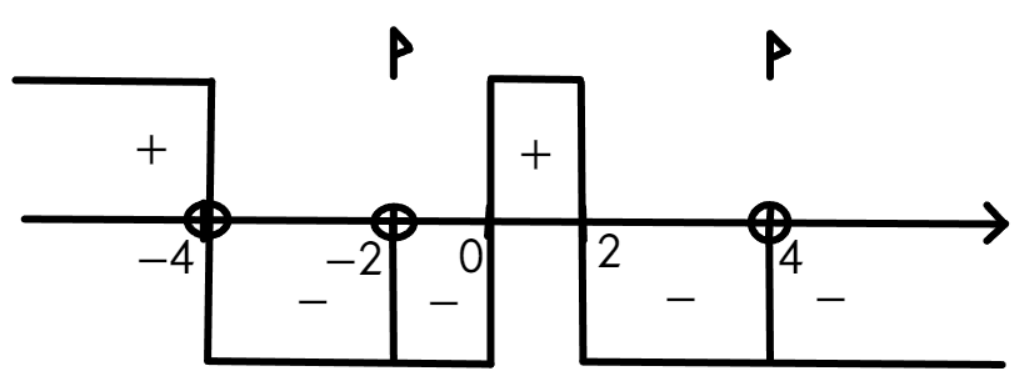
\includegraphics[scale=0.35]{ner9-3.png}}
\end{figure}\\
